% Chapter 1

\chapter{Introduction} % Main chapter title

\label{Chapter1} % For referencing the chapter elsewhere, use \eqref{Chapter1} 

\lhead{Chapter 1. \emph{Introduction}} % This is for the header on each page - perhaps a shortened title

%----------------------------------------------------------------------------------------
%\DeclareMathOperator*{\Min}{Min}
The problem addressed is to find a local minimizer of the Non-Smooth minimization problem

\begin{equation} \label{mainproblem}
  \begin{aligned}
    & \underset{x \in \mathbb{R}^n}{\text{min}}
    & & f(x) \\
    & \text{s.t.}
    & & l_i \leq x_i \leq u_i , \; \\
    & & & i = 1, \ldots, n.
  \end{aligned}
\end{equation}

where $f \colon \mathbb{R}^n \to \mathbb{R}$, is continuous but not differentiable everywhere and $n$ is large.

The \texttt{L-BFGS-B} algorithm \citep{lbfgsboriginal} is a standard method for solving large instances of \eqref{mainproblem} when $f$ is a smooth function tipically, twice differentiable. The original name of \texttt{BFGS} stands for Broyden, Fletcher, Goldfarb and Shanno, the authors
of the original \texttt{BFGS} quasi-Newton algorithm for unconstrained
optimization discovered and published
independently by them in 1970 \citep{Broyden, Fletcher, Goldfarb, Shanno}.
This method requires storing and updating a matrix which 
approximates the inverse of the Hessian $\nabla^2 f(x)$ and
hence requires $\mathcal{O}(n^2)$ operations per iteration.  
The \texttt{L-BFGS} variant \citep{MR572855}, where the \texttt{L} stands for ``Limited-Memory'' and also for ``Large'' problems, is based on \texttt{BFGS} but requires only $\mathcal{O}(mn)$ operations per iteration, and requires less memory. Instead of storing the $n \times n$ Hessian approximations, \texttt{L-BFGS} stores only $m$ vectors of dimension $n$, where $m$ is a number much smaller than $n$. Finally, the last letter B in 
\texttt{L-BFGS-B} stands for bounds, meaning the lower and upper
bounds $l_i$ and $u_i$ in equation \eqref{mainproblem}.  The \texttt{L-BFGS-B} algorithm is implemented in a FORTRAN software package \citep{lbfgsbsoftware}.

In this thesis, we first give a brief description of the \texttt{L-BFGS-B} algorithm
at a high level and then we introduce a modified algorithm which
is more suitable for functions $f$ which may not be
differentiable at their local or global optimal points.  
We call the new algorithm L-BFGS-B-NS where NS stands for
Non-Smooth.  These changes were implemented in a modified version 
of the FORTRAN code \citep{lbfgsbNS} which can be downloaded from a web repository.  We report on some numerical experiments 
that strongly suggest that the new code should be useful for the
non-smooth bound-constrained optimization problem (1.1).

We are grateful to Jorge Nocedal and his coauthors for allowing us 
to modify the L-BFGS-B code and post the modified version.  

\chapter{L-BFGS-B}
\label{ChapterConstraints} % For referencing the chapter elsewhere, use \eqref{ChapterConstraints} 

This section is a description of the original \texttt{L-BFGS-B} code \eqref{lbfgsbsoftware, codepaper} at a very high level. The original software is intended to find local minimizers of smooth functions. This thesis discusses how to modify the algorithm for Non-Smooth functions.

\section{BFGS}

\texttt{BFGS} is a standard tool for optimization of smooth functions \citep{nocedal}. It is a line search method. The search direction is of type $d = -B_k \nabla f(x_k)$ where $B_k$ is the $k^{th}$ approximation to the inverse Hessian of $f$.\footnote{When it is exactly the inverse Hessian the method is known as Newton's method. Newton's method has quadratic convergence but requires the explicit calculation of the Hessian at every single step.} This $k^{th}$ step approximation is calculated via the \texttt{BFGS} formula

\begin{equation} \label{bfgsupdate}
  \begin{aligned}
    B_{k+1} = \left(I - \frac{s_ky_k^T}{y_k^Ts_k} \right) B_k \left( I - \frac{y_ks_k^T}{y_k^Ts_k} \right) + \frac{s_k s_k^T}{y_k^T s_k}
  \end{aligned}
\end{equation}

where $y_k = \nabla f(x_{k+1}) - \nabla f(x_k)$ and $s_k = x_{k+1} - x_k$.  \texttt{BFGS} exhibits super-linear convergence on generic problems but it requires $\mathcal{O}(n^2)$ operations per iteration \citep{nocedal}.

In the case of Non-Smooth functions, \texttt{BFGS} typically succeeds in finding a local minimizer \citep{overtonlewis}. However, this requires some attention to the line search conditions. These conditions are known as the Armijo and weak Wolfe line search conditions and they are a set of inequalities used for the computation of an appropriate step length that reduces the objective function ``sufficiently''. These inequalities will be explained later in section \eqref{Wolfeconditions}

\section{L-BFGS}

\texttt{L-BFGS} stands for Limited-memory \texttt{BFGS}. This algorithm approximates \texttt{BFGS} using only a limited amount of computer memory to update the inverse of the Hessian of $f$. Instead of storing a dense $n \times n$ matrix, \texttt{L-BFGS} keeps an approximation to a record of the last $m$ iterations where $m$ is a small number that is chosen in advance\footnote{In this thesis $m < 20$, and in practice numbers between 5 and 10 are regularly used. There is no way of knowing a priory what choice of $m$ will provide the best results as will be illustrated later in this thesis}. For this reason the first $m$ iterations of \texttt{BFGS} and \texttt{L-BFGS} produce exactly the same search directions.

Because of this construction, the \texttt{L-BFGS} algorithm is less computationally intensive and requires only $\mathcal{O}(mn)$ operations per iteration. So it is much better suited for problems where the number of dimensions $n$ is large. For this reason it is the algorithm of choice in this thesis.

\section{L-BFGS-B}

Finally \texttt{L-BFGS-B} comes naturally as an extension of \texttt{L-BFGS}. The $B$ stands for the inclusion of Boundaries.  \texttt{L-BFGS-B} requires two extra steps on top of \texttt{L-BFGS}. First, there is a step called \emph{gradient projection} that reduces the dimensionality of the problem. 

Depending on the problem, the gradient projection could potentially save a lot of iterations by eliminating those variables that are at bound at the optimum reducing the initial dimensionality of the problem and the number of iterations and running time. After this \emph{gradient projection} comes the second step or \emph{subspace minimization}. During the \emph{subspace minimization} phase, an approximate quadratic model of \eqref{mainproblem} is solved iteratively in a similar way that the original \texttt{L-BFGS} algorithm is solved. The only difference is that during the search step phase the step length is restricted as much as necessary in order to remain within the $lu$-box defined by equation \eqref{mainproblem}.

\subsection{Gradient Projection} \label{gp}
The original algorithm was created for the case when $n$ is large and $f$ is smooth. Its first step is the gradient projection similar to the one outlined in \citep{gradproj1, gradproj2} which is used to determine an active set corresponding to those variables that are on either their lower or upper bounds. The active set defined at point $x^*$ is:

\begin{equation}
  \begin{aligned}
    \mathcal{A}(x^*) = \{ i \in \{1 \ldots n\} |  x^*_i = l_i \vee  x^*_i = u_i\}
  \end{aligned}
\end{equation}

Working with this active set is more efficient in large scale problems. A pure line search algorithm would have to choose a step length short enough to remain within the box defined by $u_i$ and $l_i$. So if at the optimum, a large number $\mathcal{B}$ of variables are either on the lower or the upper bound. At least a number $\mathcal{B}$ of iterations might be needed. Gradient projection tries to reduce this number of iterations. In the best case, only $1$ iteration is needed instead of $\mathcal{B}$.

Gradient projection works on the linear part of the approximation model:

\begin{equation} \label{themodel}
  \begin{aligned}
    m_k(x) = f(x_k) + \nabla f(x_k)^T ( x - x_k) + \frac{(x - x_k)^T H_k (x - x_k) }{2}
  \end{aligned}
\end{equation}

where $H_k$ is a \texttt{L-BFGS-B} approximation to the Hessian $\nabla^2 f$ stored in the implicit way defined by \texttt{L-BFGS}.

In this first stage of the algorithm a piece-wise linear segment starts on the current point $x_k$ in the direction $-\nabla f(x_k)$. Whenever this direction encounters one of the constraints, the line segment turns corners in order to remain feasible. The path is nothing but the feasible piece-wise projection of the negative gradient direction on the constraint box determined by the values $\overrightarrow{l}$ and $\overrightarrow{u}$. At the end of this stage, the value of $x$ that minimizes $m_k(x)$ restricted to this piece-wise gradient projection path is known as the ``Cauchy point'' $x^c$. See figure \eqref{caja}

\begin{figure}
\begin{center}
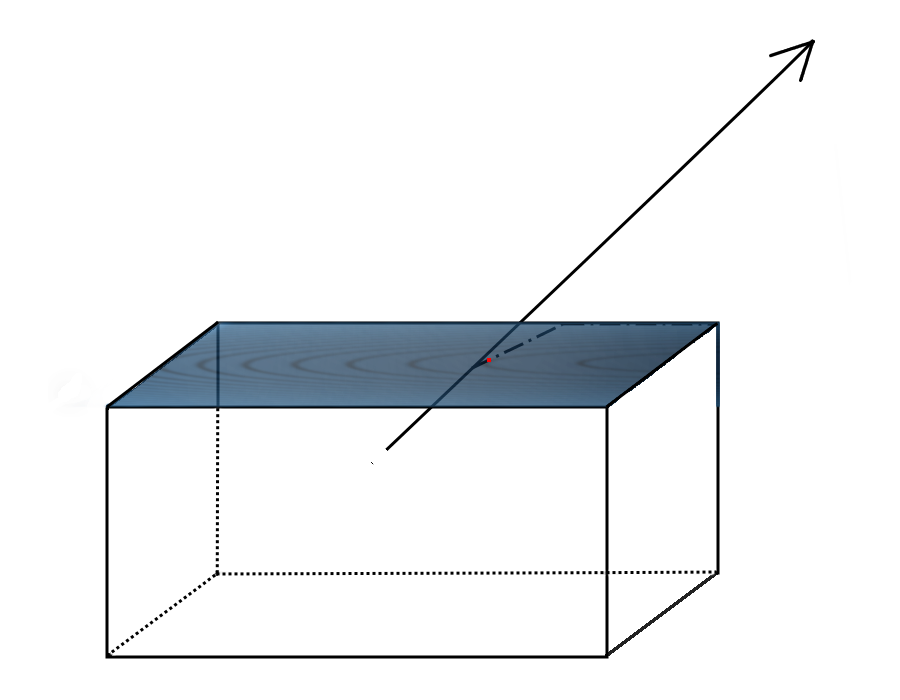
\includegraphics[scale=0.4]{Figures/cajapresentation2.png}
\caption[Graphical Representation of Gradient Projection]{The arrow represents the direction of the gradient. The dotted path represents the projected gradient path from the gradient and onto the box. The region represents the level sets of the model. The optimal point (in red) is the Cauchy point $x^c$}
\label{caja}
\end{center}
\end{figure}

\subsection{Subspace Minimization}

The problem with gradient projection is that its search direction does not take advantage of information provided implicitly by the Hessian $H_k$, and therefore the speed of convergence is at best linear. It is for this reason that a stage two is necessary. Stage 2 or subspace minimization uses an \texttt{L-BFGS} implicit approximation of the Inverse Hessian matrix restricted to the free variables that are not in the active set $\mathcal{A}(x^c)$.

The idea at a higher level is to solve the constrained problem \eqref{themodel}, but only on those dimensions that are free. The starting point for this new stage will be the previously found Cauchy point $x^c$, the \texttt{L-BFGS} algorithm provides a new search direction $\hat{d}^u$ that takes implicit advantage of second order approximations of the Hessian matrix.

The algorithm will move in the direction $\hat{d}^* = \alpha^* \hat{d}^u$ where $\alpha^*$ (the step length) is chosen so that the new point $\bar{x}_i$ satisfies Armijo and weak Wolfe descent\footnote{Armijo and weak Wolfe conditions will be explained on section \eqref{Wolfeconditions}} and curvature conditions, A third restriction on the step length is added so that the next iteration stays feasible. Once this step is finished, the next and final step will be the termination condition. If the termination condition fails, a new gradient projection and subspace minimization will be needed. If the termination condition is successful, the program exits with an appropriate exit message.

\chapter{Modifications to the L-BFGS-B algorithm}

We made three main changes to the original \texttt{L-BFGS-B} algorithm. They concern the line search Wolfe conditions, the line search methodology, and the termination condition.

\section{The Armijo and Wolfe conditions} \label{Wolfeconditions}

Probably the most important change made to the original code was the change in the curvature condition. It is accepted that the Armijo and Wolfe conditions work very well whenever the function $f$ is smooth \citep{MR1855221}. The Armijo condition, also known as the sufficient decrease requirement in the direction $d_k$ is defined as

\begin{equation} \label{armijocondition}
  \begin{aligned}
    f(x_k + \alpha_p d_k) \leq f(x_k) + c_1 \alpha_k d_k^T \nabla f(x_k)
  \end{aligned}
\end{equation}

where $0 < c_1 < 1$ is a constant usually $c_1 = 10^{-4}$ \citep{nocedal}. This condition guarantees that the function continues decreasing and eventually reaches some optimum. It is possible to continue decreasing without ever reaching the optimum if the armijo condition is not required as is shown in figure~\eqref{armijograph}

\begin{figure} 
\begin{center}
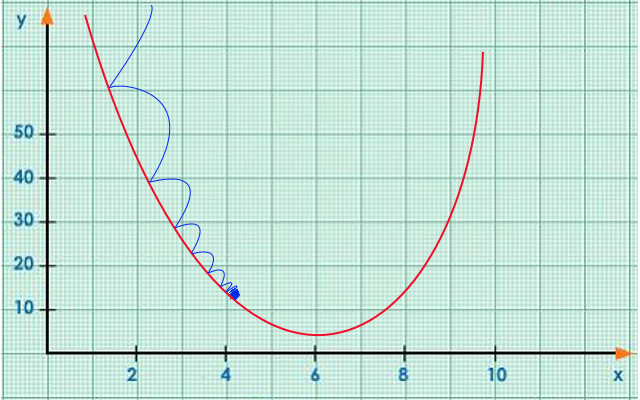
\includegraphics[scale=0.5]{Figures/armijo.png}
\caption[Representation of the Armijo Condition in a Nutshell]{In this figure, the iterations always reduce the value of the function a little bit, but never enough to go below $12$}
\label{armijograph}
\end{center}
\end{figure}

The other condition and the one that was actually changed, is the curvature condition, of which the most popular version is the ``strong Wolfe'' curvature condition:

\begin{equation} \label{strogWolfeq}
  \begin{aligned}
    |d_k^T \nabla f(x_k + \alpha _k d_k)| \leq c_2 |d_k^T \nabla f(x_k)|
  \end{aligned}
\end{equation}

Where $d_k$ represents the search direction and $c_2$ is a constant such that $0 < c_1 < c_2 < 1$ and is usually $c_2 = 0.9$ \citep{nocedal}. The strong Wolfe condition is a natural choice for optimization of smooth functions. Its goal is to find a step length long enough that the slope has been reduced ``sufficiently'' as illustrated in figure~\eqref{Wolfefigure}, but the problem is that the condition as it is, does not work well for the Non-Smooth case. This is because near the minimal points there may be abrupt changes in the gradient. a good example of this problem is the function $f(x) = |x|$, where the slope never becomes flat near the optimal point.

\begin{figure} 
\begin{center}
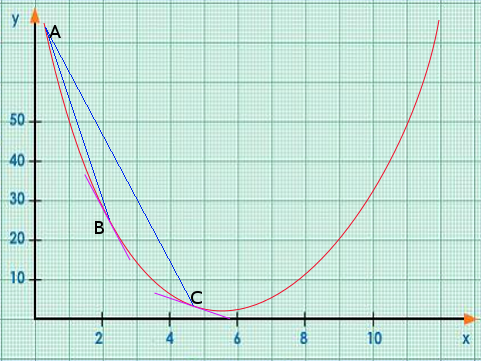
\includegraphics[scale=0.65]{Figures/wolfe.png}
\caption[The Idea behind the Wolfe Condition]{The logic of Wolfe conditions is this. Starting at point A. Point B is a step in the right direction, however, point C offers a ``flatter'' tangent and should be closer to the optimum which has a tangent of zero (Smooth case)}
\label{Wolfefigure}
\end{center}
\end{figure}

The weak Wolfe condition defined as

\begin{equation}
  \begin{aligned}
    d_k^T \nabla f(x_k + \alpha _k d_k) \geq c_2 d_k^T \nabla f(x_k)
  \end{aligned}
\end{equation}

can be used in the Non-Smooth case. It is all that is needed to guarantee that the \texttt{BFGS} updated inverse Hessian approximation is positive definite \citep{overtonlewis}. This weak version is suited for the problems in this thesis and it was implemented as part of the line search algorithm explained in the next section.

\section{The Line Search Methodology}

The original \textsc{FORTRAN} software \citep{lbfgsbsoftware} contains a line search subroutine. This subroutine originally consisted of three steps. A maximum length,a sufficient decrease and a curvature condition (the Armijo and Wolfe conditions from the previous section). This sub-procedure was partially changed for the purpose of this thesis. The old version of the code was not removed, it was left commented out and is only explained here with the purpose of showing why it needed to be modified. It was called on line $2662$ \eqref{ignoredcode} of \texttt{lbfgsbnomessages.f90} which is a file within the github repository \citep{lbfgsbNS}.

\begin{enumerate}
\item[1^{st}] The line search requires a maximum step. This maximum step is such that it guarantees that the step length stays within the bounding box delimited by $l$ and $u$, as such, this is a unique feature of the bounded algorithm\texttt{L-BFGS-B}. In the original \textsc{FORTRAN} code, this part of the line search was not changed.

\item[2^{nd}] An interval for $\alpha_k$ is chosen so that it contains a minimizer of the modified function,

\begin{equation} \label{armijomod}
  \begin{aligned}
    \Psi(\alpha_k) = f(x_k + \alpha_k d_k) - f(x_k) - c_1 \alpha_k d_k^T  \nabla f(x_k)
  \end{aligned}
\end{equation} 

 which is nothing but a modification of the Armijo condition \eqref{armijocondition}. If $\Psi(\alpha_k) < 0$ and $\alpha_k d_k^T \nabla f(x_k) > 0$. The interval contains a minimizer of $f$ and the subroutine can continue to the next step. This first stage took place in the subroutine $dcsrch$; specifically on lines $3687$ and $3709$ on appendix \eqref{stage2}.

\item[3^{rd}] This stage is very similar to the typical line search \citep{nocedal}. It was called on line $3713$ of \texttt{lbfgsbnomessages.f90} and its mission was to find the step that satisfied Armijo and ``Strong'' Wolfe conditions on the original function $f$. Both steps 2 and step 3 are called on the subroutine $dcstep$. The subroutine still exists on file \texttt{lbfgsbnomessages.f90} for illustration. Although it is only commented out and never called in this thesis.

\end{enumerate}

Those three steps make up the original subroutine. But there is a problem with the function $dcstep$ on the third step as it concerns this thesis. It turns out that function $dcstep$ was designed to work only with smooth functions in mind. The algorithm takes advantage of quadratic and cubic approximations to the function in order to calculate step lengths that satisfy Armijo and Wolfe conditions. Unfortunately, these second and third order approximations do not work in the Non-Smooth case, and the optimizer crashes under the line search as it is. Function $dcstep$ starts on line $3779$ and a sample of the approximations is shown in between lines $3881$ and $3902$ of appendix \eqref{nsnowork} of \texttt{lbfgsbnomessages.f90}.

The solution to this particular issue is to use a line search similar to the one implemented in hanso \citep{hanso}. The HANSO approach is to double the step length while the Armijo condition is violated. And once the interval has been bracketed, to do a bisection until both Armijo and Wolfe conditions are satisfied. The only difference with the HANSO approach in this thesis is that the line search in HANSO can double its step length up to $30$ times\footnote{for all practical purposes this is considered a good limit of iterations}. Whereas in this thesis, the step length can double only as long as the step length is less than the maximum value that guarantees feasibility of the solution (the maximum established in the first step of the original line search). This version of the bisection and expansion is found in between lines $4425$ and $4456$ of \texttt{lbfgsbnomessages.f90} in appendix \eqref{linesearchww} 

\section{The Termination Condition} \label{terminator}

One important requirement of an algorithm is that it ends in a finite time. In the case of smooth functions, \texttt{L-BFGS-B} checks whether the algorithm has converged, by means of the \emph{projected gradient}\footnote{Not to be confused with ``gradient projection'' from subsection \eqref{gp}} which is nothing but the projection of the negative gradient onto the bounding box defined by $l$ and $u$. If this projected gradient has a small norm\footnote{smaller than some tiny $\epsilon > 0$} the algorithm has converged. In the case of Non-Smooth functions however, this is not necessarily true and the function at the minimum may have a wedge. In this wedge the projected gradient may not vanish. Furthermore, if there is a sequence of points that approaches the optimum $x$ in a direction $\vec{p}$, the projected gradients corresponding to this sequence of points might be completely different from the projected gradients associated to a sequence of points that approach the optimum $x$ from an opposite direction.

Given this set of conditions, there is a need for particular rules to establish the finalization of the optimization, these rules have already been established in some works before \citep{overtonlewis, skajaa}.

\subsection{Termination Condition Sub-algorithm}
%Warning review
Overton and Lewis formulate an algorithm that gives a practical solution to this problem on section $6.3$ \citep{overtonlewis}
The best practical methodology should be to calculate whether zero $0$ or a very small number is the norm of a vector that is part of the convex hull of gradients evaluated at points near the optimum candidate $x$. The neighborhood is defined as those points with a distance to $x$ smaller than a small tolerance $\tau_x > 0$ and no more than $J \in \mathbb{N}$ iterations back in history. In order to make sure that the gradient zero $\vec{0}$ or a vector with a very small norm smaller than a very tiny tolerance $\tau_d > 0$ is part of the convex hull calculated near a neighbourhood of the optimum, the algorithm  keeps a record of the latest gradient vectors in this small neighbourhood of the point where the optimum is suspected to be located. This list of gradients is referred to as the set $\mathcal{G}$ \citep{overtonlewis}

With this list $\mathcal{G}$ of gradients at hand. The next step is to find the vector with the minimal norm contained in the convex hull of these gradients.  If the norm of this vector has a norm smaller than $\tau_d$ , the algorithm ends with a message of convergence success ``CONVERGENCE: ZERO\_GRAD\_IN\_CONV\_HULL''. If the minimum such norm is larger than the tolerance, the algorithm must continue to the following iteration and not terminate.

In order to find this vector, there is the need to solve a quadratic problem. Every vector in the convex hull can be expressed as a non-negative linear combination $Gz$ of those vectors in $\mathcal{G}$. Where $G$ is the matrix with columns made up of gradients in $\mathcal{G}$; and $z$ is such that $\sum_{i=1}^n z_i = 1$ and $z_i \geq 0$.

The objective is to find the right combination of $z$ that minimizes the norm $||Gz||_2$.  This is equivalent to solving the following optimization problem

\begin{equation} \label{quadraticproblem}
  \begin{aligned}
    & {\text{min}}
    & & q(z) = ||G z ||_2^2 = z^TG^TGz  \\
    & \text{s.t.}
    & & \sum_{i = 1} ^J z_i = 1 \; \\
    & & & z_i \geq 0.
  \end{aligned}
\end{equation}

The solution to this problem $z^*$ has the associated vector $Gz^*$. And if $||Gz^*||_2 < \tau_d$ the algorithm converges.

\subsection{The Solution of the Quadratic Program}

The solution of equation \eqref{quadraticproblem} was implemented with a practical primal-dual methodology. This methodology is the same methodology implemented by Skajaa \citep{skajaa} in his thesis. His code \textsf{qpspecial} was implemented in \textsc{FORTRAN} for this thesis and is part of \texttt{lbfgsbnomessages.f90}. His algorithm solution is the well known Mehrotra's Predictor-Corrector algorithm implementation applied to quadratic programming.

This algorithm initially tries to solve the Karush-Kuhn-Tucker $KKT$ conditions. The $KKT$ is a system of equations whose solution characterizes the solution of the original optimization problem in equation \eqref{quadraticproblem}, the Karush-Kuhn-Tucker equations are:

\begin{equation} \label{kkt}
  \begin{aligned}
    G^TGz - e^Ts
    & = & 0 & \\
    \sum_{i = 1}^J x - 1
    & = & 0 & \\
    z_is_i & = & 0 &; &i = 1,2, \dots, J\\
    (s, z) & \geq & 0 &
  \end{aligned}
\end{equation}

Where $s$ is the variable that represents the dual associated problem.

In order to solve this system of equations a variant of Newton's method is used. The method provides a search direction and as usual for this type of methods, it  requires a corresponding step length. Since this is an interior point method, it approaches the solution following a path inside the convex interior of the feasible set.  In the best of cases, it would be nice to approach the solution through a \emph{central path} defined as third equation in \eqref{kkt} is allowed to take more relaxed values $z_is_i = \tau$, where $\tau \geq 0$. If the solution is approached through this \emph{central path}. The convergence will require fewer iterations\footnote{The reason why the central path is so convenient is more thoroughly explained in Nocedal's text chapter $14$ \citep{nocedal}}. The logic is that by being central, it is kept away from the borders.

The problem with a pure Newton's method is that it's solution is not close to this \emph{central path}. The step length is usually very small because of the nature of the third and fourth equations. For this reason, if the step length is too large, either the condition of $z > 0$ or $s > 0$ will be violated. Unfortunately the pure method this way, does not allow reasonable step sizes in practice. The method approaches the solution very close to the boundaries of the feasible set and far away from the \emph{central path} where the step lengths could be larger and the convergence therefore would be faster. It is for this reason that a \emph{centering} of the path is performed. This first step is known as the ``predictor'' step.

Besides the centering; Mehrotra proposed a ``correction'' stage which pushes the solution even closer to the \emph{central path} by taking into account its curvature. This second stage is also used to calibrate some of the parameters used during the centering in the ``predictor'' stage\footnote{These are some parameters that calibrate the speed at which the tangent path is pushed into the central path. This is also explained in chapter $14$ \citep{nocedal}}. The second stage is similar to the first stage in that it requires the solution of a new system of equations.

\begin{figure}
\begin{center}
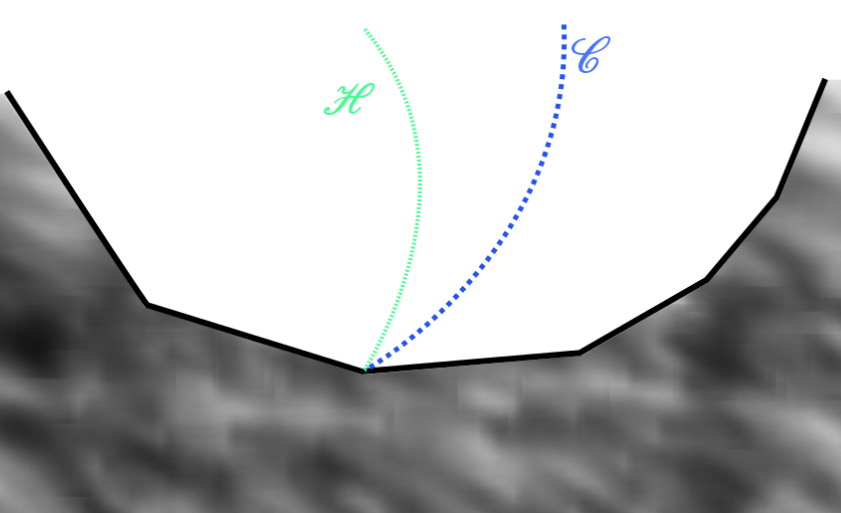
\includegraphics[scale=0.3]{Figures/CentralPath.png}
\caption[The Central Path and the Tangent Path]{The central path $\mathcal{C}$ is approached from a current and non-central point on the tangent path $\mathcal{H}$}
\end{center}
\end{figure}

And this is very important, because both steps require a solution of a system of equations which in turn requires a matrix factorization. And this factorization can be recycled. Mehrotra's algorithm requires only one Cholesky factorization for the first stage. This factorization is reused during the second stage. And reusing the factorization, the performance is improved.

\chapter{Solution Tests}

The \texttt{L-BFGS-B} implementation was tested on the high performance cluster machines at NYU. In order to run these tests it was necessary to create a series of PBS files\footnote{PBS stands for Portable Batch System. This is a software that performs job scheduling. It is used by High Performance Computing at NYU (and many other High Performance Computing Centers) to allocate computational tasks. In order to run jobs at the high performance clusters, a series of PBS batch files need to be created} using the PBS generator script on appendix \eqref{pbsgenerator}. This script generator created PBS files which in turn run bash shell scripts\footnote{Bash is a command processor. Each Bash script that was created includes a series of computer commands. In this case, the program execution of the original \texttt{L-BFGS-B} software and \texttt{L-BFGS-B-NS}}. One of them is available on appendix \eqref{pbsfile}. The main reason to run scripts this way is because it achieves parallelism, and because the system sends confirmation e-mails and statistics about the different stages of the processes giving a lot of control to the practitioner. The original \texttt{L-BFGS-B} optimizer displays different messages depending on the initial condition that triggered the exit.  

\section{Exit Messages}

The following is a list of some of the other most common exit messages in the original \texttt{L-BFGS-B} optimizer.

\begin{itemize}

\item ``ABNORMAL\_TERMINATION\_IN\_LNSRCH'' This message means that there was a problem and the program's exit was premature. It is typically found in Non-Smooth functions where the cubic interpolation is impossible. But the message is also symptomatic of other problems.

\item ``CONVERGENCE: NORM\_OF\_PROJECTED\_GRADIENT\_LT\_PGTOL": Means that convergence was achieved because the norm of the projected gradient is small enough. Notice that this convergence message does not apply to \texttt{L-BFGS-B-NS} because of particular requirements for Non-Smooth functions involving the convex hull instead as explained in section \eqref{terminator}.
\item ``CONVERGENCE: REL\_REDUCTION\_OF\_F\_LT\_FACTR*EPSMCH": This convergence condition is achieved whenever the relative reduction of the value of function $f$ is smaller than a predefined factor times machine $\epsilon$. This exit message does not apply to \texttt{L-BFGS-B-NS} either.

\item ``ERROR: N .LE. 0": This is one of many error checks performed at the beginning of the execution. This one in particulars tests positivity of the dimensionality of the problem.

\item ``ERROR: NO FEASIBLE SOLUTION": An error condition for those cases when the solution is not feasible. This is because the original \texttt{L-BFGS-B} optimizer allows open boxes of type [$l$, $\infty$[, ]$-\infty$, $u$] and ]$-\infty$, $\infty$[

\item ``WARNING: ROUNDING ERRORS PREVENT PROGRESS": If there is a rounding error issue

\end{itemize}

on top of these messages, \texttt{L-BFGS-B-NS} introduced a new message for a successful exit from its termination condition.

\begin{itemize}
\item ``CONVERGENCE: ZERO\_GRAD\_IN\_CONV\_HULL" What this means is that all termination conditions established on section \eqref{terminator} were satisfied\footnote{This does not mean that the resulting vector is exactly equal to zero $0$, but it is small enough to finish the execution of the algorithm}.
\end{itemize}

\section{Modified Rosenbrock Function} \label{ros}

With those tools in hand, it is possible to run a few tests of the algorithm. Several functions were evaluated. One of them is a modified version of the Rosenbrock function problem \citep{rosenbrock}:

\begin{equation} \label{modifiedrosenbrock}
    f(x) = (x_1 - 1)^2 + \sum_{i = 2}^n |x_i - x_{i - 1}^2|^p
\end{equation}

Here, the properties of the function depend on the value of the $p$ parameter\footnote{The original Rosenbrock function would have a value of $p = 2$ and the second term is multiplied by $100$}. This function can be proven to be locally lipschitz continuous whenever $p \geq 1$. In particular it is Locally Lipschitz continuous if restricted to a finite domain of the type $l$, $u$, similar to the one defined on equation \eqref{mainproblem}.

The region to be tested is defined by the ``box'' with boundaries

\begin{equation}
  \begin{aligned}
    x_i = 
    \begin{cases}
      [-100, 100] & \text{if } i \in \text{ even numbers} \\
      [10, 100] & \text{if } i \in \text{ odd numbers}
    \end{cases}
  \end{aligned}
\end{equation}

And the initial point was chosen to be the midpoint of the box, plus a different small perturbation for each dimension, chosen so that the line search does not reach the boundary of several dimensions in one stroke.

\begin{equation}
  \begin{aligned}
    x_i = \frac{u_i + l_i}{2} - \left(1 - 2^{1 - i}\right)
  \end{aligned}
\end{equation}

The problem is smooth for values of $p$ close to $2$, but as the values of $p$ approach $1$, the original \texttt{L-BFGS-B} optimizer should start to have problems. In order to check for that, we plug the Modified Rosenbrock function into the original \texttt{L-BFGS-B} optimizer with $p$ parameter varying between $2$ and $1$. 


\begin{figure}
\begin{center}
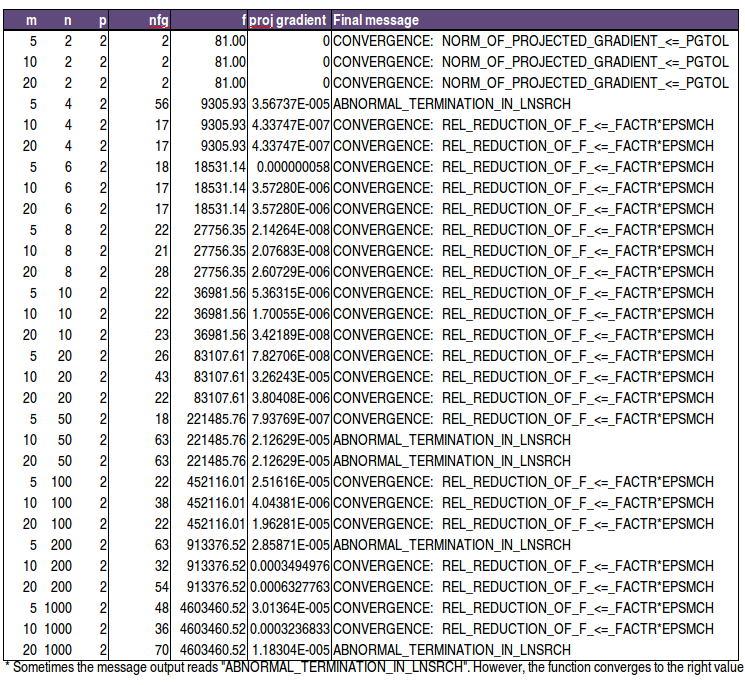
\includegraphics[scale=0.58]{Figures/Nocedalp2.png}
\caption[Modified Rosenbrock with $p = 2$]{Satisfactory results for the original algorithm \texttt{L-BFGS-B} applied to the Modified Rosenbrock function with $p = 2$}
\label{pequal2}
\end{center}
\end{figure}


For a value of $p = 2$, the original \texttt{L-BFGS-B} optimizer does not have too many problems and it yields good results as seen on the resulting table \eqref{pequal2}.

\subsection{Performance of \texttt{L-BFGS-B}}

This exercise tested three different values of $m$, where $m$ stands for the steps in memory of \texttt{L-BFGS}. The steps that were tested are $5$, $10$ and $20$, these values of $m$ cover more or less the set of recommended values. The number of dimensions in this exercise in particular ranges from $2$ to $1000$ and covering many values in between. The column $nfg$ stands for the number of iterations taken in order to finish the algorithm and $f$ stands for the optimal value that was achieved during the optimization. The two last columns stand for the norm of the projected gradient and the final message when the algorithm finished.

In all cases the projected gradient has a very small norm. When this norm is tiniest the convergence is achieved because the norm of the projected gradient is smaller than the threshold. In other cases, the program exits successfully after a relative reduction in the size of the function. In other cases, an abnormal termination message is sent to the output.

Notice that in \eqref{pequal2} the program sometimes sends an ``ABNORMAL\_TERMINATION\_IN\_LNSRCH'' warning message even though the function has converged to a value that is very close to the optimal expected value.  This is because the original Rosenbrock function is designed to be very difficult to solve.  Its minimum is located in the middle of a banana shaped valley. This valley is very flat and is designed to be a test problem that causes trouble to even the best optimizers as. The shape of the original Rosenbrock function can be seen in figure \eqref{dualgraph}. The shape of this region is perhaps easier to see on the contour plot \eqref{contourbanana}. The minimum is locate at the point ($1$, $1$) on one of the corners.

\begin{figure}
\centering
\mbox{\subfigure{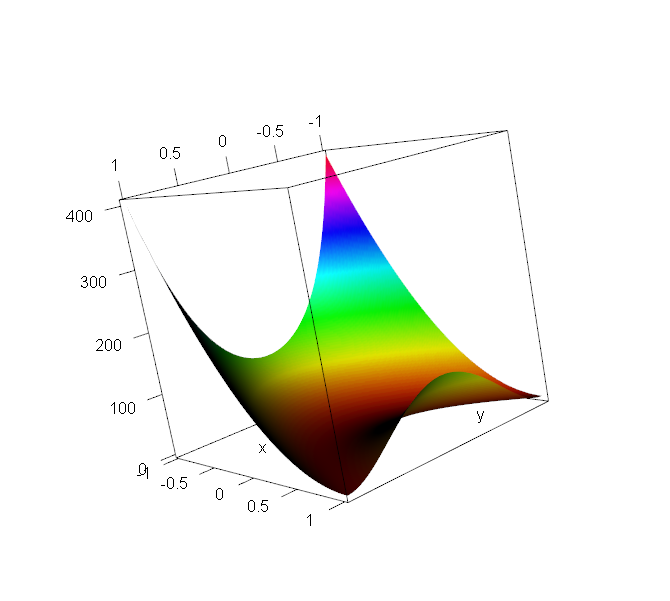
\includegraphics[scale = 0.4]{Figures/rosenbrock.PNG}} \quad
\subfigure{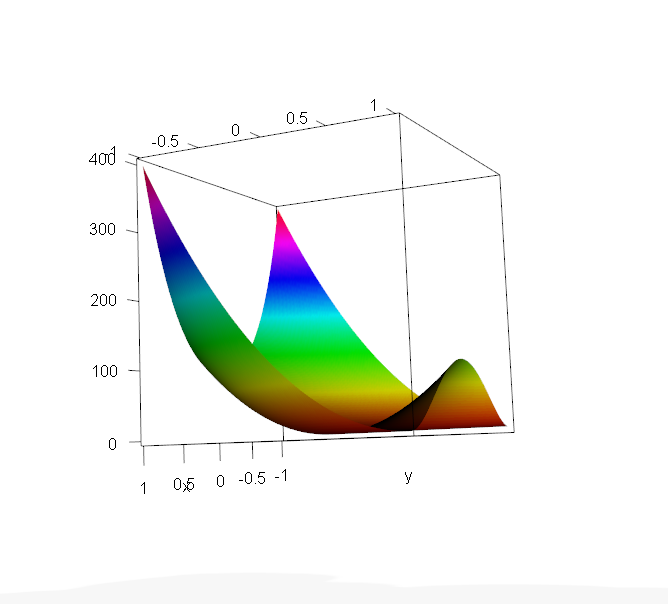
\includegraphics[scale = 0.4]{Figures/FlatBottom.PNG} }}
\caption[Original Rosenbrock Function Mesh]{The original Rosenbrock function $f(x,y) = (1 - x)^2 + 100(y - x^2)^2$ is designed to be a very difficult function to optimize. The global minimum is located along the very narrow, flat banana shaped valley \citep{rosenbrock}}
\label{dualgraph}
\end{figure}

\begin{figure}
\begin{center}
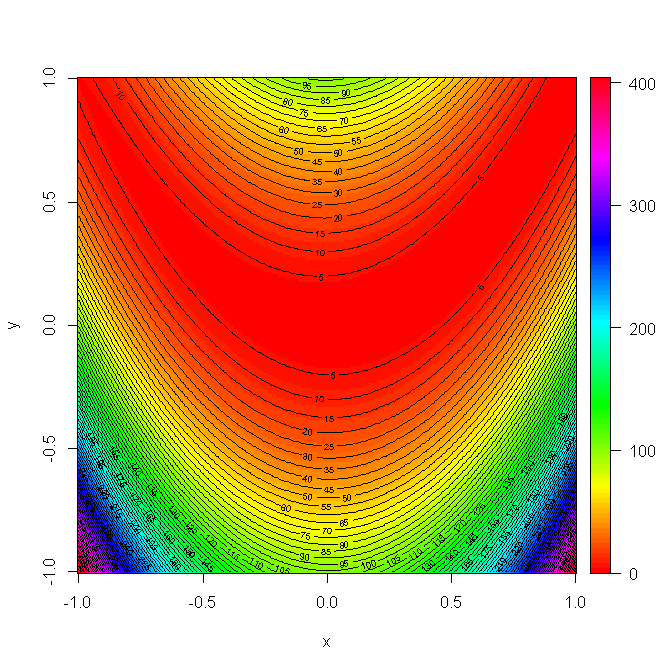
\includegraphics[scale=0.5]{Figures/contour.PNG}
\caption[Contour Plot of the Original Rosenbrock Function]{The contour plot shows the valley in red where the global optimum is located. It is located at the corner on (1, 1)}
\label{contourbanana}
\end{center}
\end{figure}

The overall conclusion from this exercise is that the original \texttt{L-BFGS-B} optimizer works well, for the smooth modified Rosenbrock case\footnote{The original algorithm solves a modified version of this function \eqref{modifiedrosenbrock} with parameter $p = 2$, so it is to be expected that the performance is good}.

\begin{figure}
\begin{center}
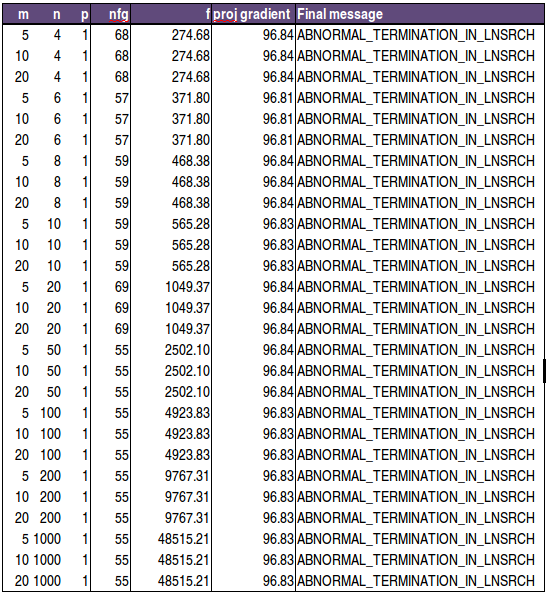
\includegraphics[scale=0.5]{Figures/abnormalNocedal.png}
\caption[Modified Rosenbrock with $p = 1$]{Unsatisfactory results for the original algorithm \texttt{L-BFGS-B} applied to the Modified Rosenbrock function with $p = 1$, notice however that the two-dimensional case is successful.  This is because the function is smooth in this particular case.}
\label{pequal1}
\end{center}
\end{figure}

On the other hand, the value of $p = 1$ has an abnormal line search termination in most of the cases presented. The projected gradient values are always far away from zero see table \eqref{pequal1}. 

In this exercise, the memory length $m$ of \texttt{L-BFGS}, does not have an impact on the final value $f$ of the optimization, but this is because all cases crashed before the $5^{th}$ iteration and therefore all different cases of $m$ end up looking exactly the same in this table.

But an analysis of only the values $p = 1$ and $p = 2$ would not be enough. And therefore several other values of $p$ were also tested, among others $1.5$, $1.1$, $1.01$, $1.001$, ... , $1.000000001$, $1$. As expected, those values where $p$ is closer to $1$ are the most difficult to solve for the original algorithm. When $p=1$ the algorithm does not work as seen in \eqref{pequal1}\footnote{This is expected because the algorithm is originally designed to handle only smooth functions}. It is important to point out that the two dimensional case is successful because in this particular case the function is smooth inside its bounding box.

\subsection{Performance of \texttt{L-BFGS-B-NS}}

For intermediate values, the new changes seem to provide better values of $f$. Here is a simple comparison of the algorithm running on $m = 5,10$ for selected values of $p$ \eqref{pcomp}

\begin{figure}
\begin{center}
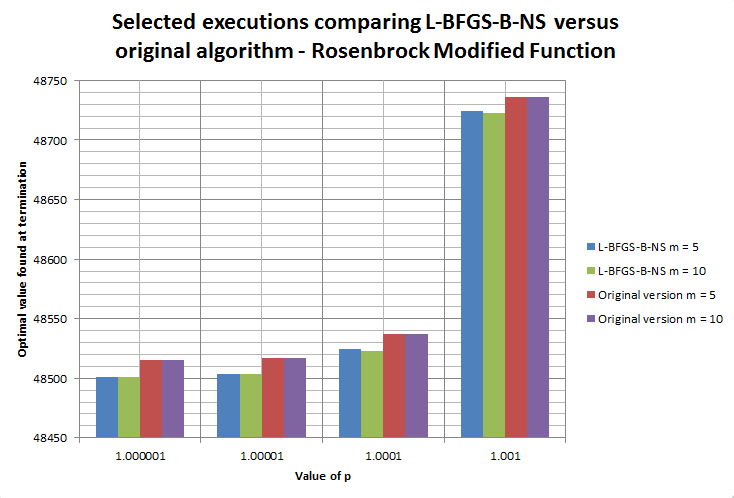
\includegraphics[scale=0.75]{Figures/ComparisonNewOld.PNG}
\caption[Comparison of selected values of the Modified Rosenbrock function]{Comparison of the performance of \texttt{L-BFGS-B-NS} vs. the Original version of \texttt{L-BFGS-B} applied to the Modified Rosenbrock function with selected values of p in 1.000 dimensions}
\label{pcomp}
\end{center}
\end{figure}

These are typical values of optimizations for intermediate values of $p$. In the bar graph it is possible to see that values generated via \texttt{L-BFGS-B-NS} are a little better for values of $p$ closer to $1$. 

The test performed is represented in a table with the number of iterations performed sliced by $p$ and $m$ \eqref{pmtableiter}. And just as it would be expected, the number of evaluations required is higher for values of $p$ close to $1$.

\begin{figure}
\begin{center}
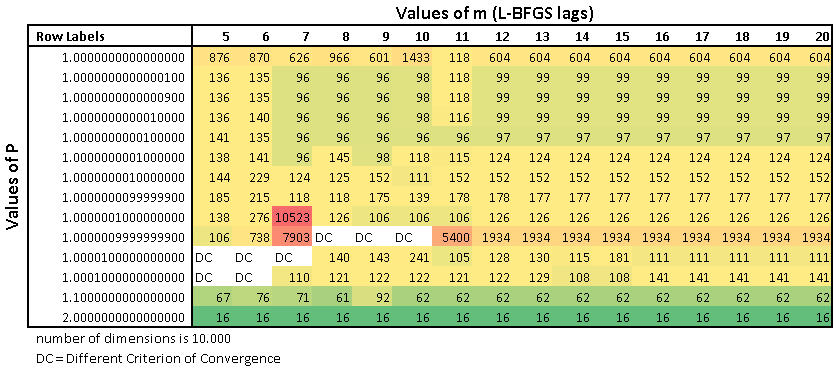
\includegraphics[scale=0.55]{Figures/Niterations.PNG}
\caption[Number of function iterations for different values of $p$ and $m$ in the solution of Modified Rosenbrock]{This is the number of iterations for different values of $p$ and $m$. Blank values converged using other stopping criteria besides the termination condition on \eqref{terminator}}
\label{pmtableiter}
\end{center}
\end{figure}

The same table is reported for the number of function evaluations (as opposed to number of iterations) required to achieve convergence on table \eqref{pmtable}

\begin{figure}
\begin{center}
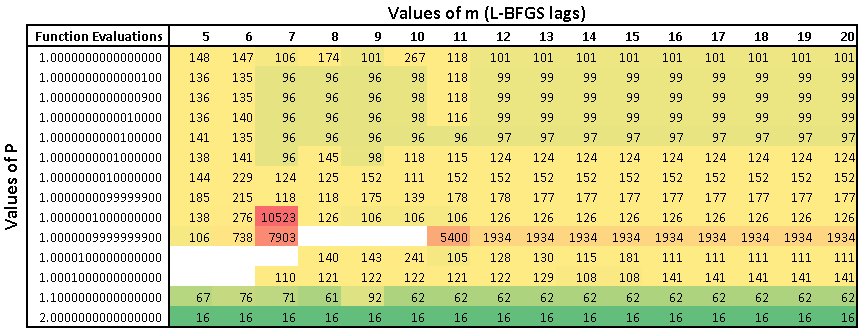
\includegraphics[scale=0.55]{Figures/Nevaluations.PNG}
\caption[Number of function evaluations for different values of $p$ and $m$ in the solution of Modified Rosenbrock]{This is the number of function evaluations for different values of $p$ and $m$. The number of function evaluations is a few times higher than the number of iterations because each iteration requires to evaluate the function a couple of times for the line search. Blank values converged using other stopping criteria besides the termination condition on \eqref{terminator}}
\label{pmtable}
\end{center}
\end{figure}

The values on these tables should be compared with the much more difficult problem in the next section.

\section{Nesterov's Chebyshev-Rosenbrock Modified function}
The original \texttt{NCR-NS1} function was first introduced in the thesis by Kaku \citep{kaku}. It is a Non-Smooth variation of the \texttt{NCR} function. In this thesis there is yet a newer modification to this function and it is defined very similar to the function \eqref{modifiedrosenbrock}. with the inclusion of a $p$ parameter.

\begin{equation} \label{modifiedyurirosen}
    f(x) = \frac{(x_1 - 1)^2}{4} + \sum_{i = 1}^{n-1} |x_{i+1} - 2x_{i}^2 + 1|^p
\end{equation}

And just like in equation \eqref{modifiedrosenbrock} $p$ is also assigned as a control variable for the Lipschitz Continuity of the function. The problem as stated in Kaku's thesis, is that the manifold defined by the term inside the sum,

\begin{equation} \label{kakumanifold}
    M = \{x: x_{i+1} - 2x_i^2 + 1 = 0, i = 1, \hdots, n-1 \}
\end{equation}

is highly oscillatory in nature, and therefore \texttt{BFGS} type of methods require many iterations to converge. In particular, table \eqref{yuripn} tries to slice the number of iterations required to finish the algorithm given different combinations of $p$ and $n$, the number of dimensions. See table \eqref{yuripn}.

\begin{figure}
\begin{center}
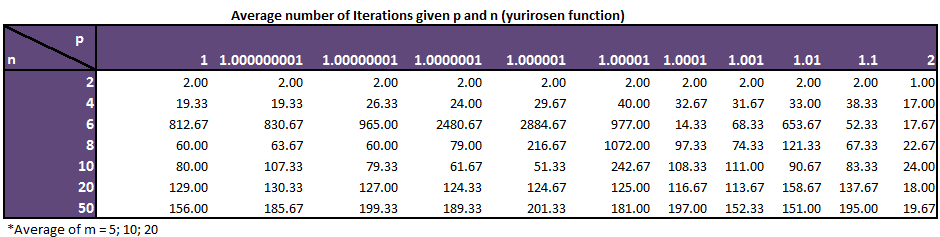
\includegraphics[scale=0.6]{Figures/yurirosenpn.PNG}
\caption[Comparison of selected values of the Modified NCR-NS1 function pivoting by p and n parameters]{Comparison of the number of iterations in order to converge for the Modified NCR-NS1 functions sliced by the number of dimensions $n$ and the $p$ parameter that controls the Smoothness of the function}
\label{yuripn}
\end{center}
\end{figure} 

The results show that the number of iterations increases significantly with smaller values of $p$ and with larger values of the dimension $n$. Also, the number of iterations is a lot larger than for the previous case on section \eqref{ros}. 

This table was also pivoted with parameters $n$ and $m$ in table \eqref{yurimn}. And again you can see that the complexity of the problems grows with variable $n$, but there is no clear trend on the influence of $m$ in the speed of convergence.

\begin{figure}
\begin{center}
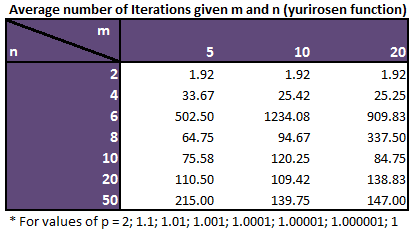
\includegraphics[scale=0.9]{Figures/yurirosenmn.PNG}
\caption[Comparison of selected values of the Modified NCR-NS1 function pivoting by m and n parameters]{Comparison of the number of iterations in order to converge for the Modified NCR-NS1 functions sliced by the number of dimensions $n$ and the memory lag $m$}
\label{yurimn}
\end{center}
\end{figure} 

\chapter{Conclusions}

%-------------------------------------------------------------------------
The need to build optimizers that work on a large number of variables quickly. Led us to the use of large scale quasi-Newton methodologies. These methodologies have been shown to work very well for smooth functions and several implementations have been suggested and made available already.

In the case of Non-Smooth functions, a lot of changes were proposed in this thesis. Implementing the changes proposed to the original \texttt{L-BFGS-B} software provides the capability to run optimizations on Non-Smooth functions on simply restricted domains. The most important changes were the Wolfe condition; which was changed from the strong to the weak version and using a line search algorithm that does not require smoothness of the function at critical points.

With the new tool, which is called \texttt{L-BFGS-B-NS}, it is possible to run optimizations of problems in large dimensions for some complicated tests. The software has been tested with very challenging functions and has performed well.

The new methodology offered some challenges to the way in which the algorithm terminates and for this reason it was also necessary to implement termination conditions that take care of the wedges natural to Non-Smooth functions. The new termination conditions work fine for the problems tested.

After running the algorithm it seems like there is not a good rule to choose the number of memory step terms $m$ to keep in memory, but this is something that also happened in the case of smooth functions. Also, the test functions Modified Rosenbrock and Modified NCR-NS1, show that the more ``Non-Smooth'' a function becomes, the more iterations and function evaluations will be required for the function to converge.

Another conclusion, quite obvious, is that larger problems involve a greater number of resources

Future steps suggest the investigation of limited-memory bundled methods $LMBM$, how it compares with \texttt{L-BFGS-B-NS} and how one could benefit from the other. Also, the study of the impact of the Lipschitz constant on the convergence of the \texttt{L-BFGS-B-NS} algorithm \citep{QJ:QJ935}. This line of research opened up as we were already finishing this thesis.

